\documentclass[a4paper]{article}

\usepackage[portuguese,english]{babel}
\usepackage[utf8]{inputenc}
\usepackage[T1]{fontenc}

\newcommand{\documentTitle}{Software Reuse \\ Final Project}
\newcommand{\pdfTitle}{Software Reuse: Final Project}
\newcommand{\documentAuthors}{João Rafael (2008111876, jprafael@student.dei.uc.pt) \\ José Ribeiro (2008112181, jbaia@student.dei.uc.pt)}

\title{\documentTitle}
\author{\documentAuthors}

\usepackage{hyperref}
\hypersetup{
	pdftitle = \pdfTitle
	,pdfauthor = \documentAuthors
	,pdfsubject = {Software Reuse: Final Project}
	,pdfkeywords = {Software Reuse} {Design Patterns}
	,pdfborder = {0 0 0}
}

\usepackage{subfig}
\usepackage{amsmath}
\usepackage{array}
\usepackage{anysize}
\usepackage{lscape}
\usepackage[pdftex]{graphicx}
\usepackage[table]{xcolor}
\usepackage{caption}
\usepackage{pdfpages}

\marginsize{3.5cm}{3.5cm}{3cm}{3cm}

\makeatletter

\begin{document}
\renewcommand{\figurename}{Figure}
\maketitle
\cleardoublepage

\tableofcontents
\cleardoublepage

\setlength{\parindent}{1cm}
\setlength{\parskip}{0.3cm}

\hyphenation{}

% \begin{center}
% 	\includegraphics[width=1.00\textwidth]{images/peak.png}
% 	\captionof{figure}{QRS complex detection.}
% 	\label{fig:peak}
% \end{center}

\section{Introduction}
\noindent No âmbito da cadeira de Reutilização de Software, foi-nos dada a oportunidade de realizar um projecto segundo a metodologia de Extreme Programming, e pedida uma análise sobre o impacto da aplicação de Padrões de Projecto no desenvolvimento no projecto. Estes são os resultados.


\section{Architecture Overview}
\subsection{GUI}

No inicio da aplicação cria-se um \emph{widget} \texttt{BreakoutLauncher}. Neste, é possível escolher o nível a jogar, definido num ficheiro em formato JSON, e os dois participantes. Ao escolher estas definições é criada a janela principal do jogo \texttt{BreakoutGame} que contém um \texttt{BreakoutFrame}. Em conjunto estes dois objectos permitem a visualização e interação com o estado do jogo \texttt{BreakoutWorld}.

\subsection{Physics}
O \emph{namespace} \texttt{physics} engloba as classes relativas ao motor de física. O mundo, caracterizado pela classe abstracta \texttt{World}, permite a interacção de objectos \texttt{Body}. Dois tipos primitivos de objecto são suportados: \texttt{Body} e \texttt{Circle}. Por si, estes objectos não modelam o conceito de velocidade, existindo para este efeito a classe \texttt{Movable} que pode ser utilizada através de herança múltipla. A cada \emph{step} são actualizadas as posições dos objectos, e procede-se a detecção de colisão. Para tal são utilizadas as funções definidas como \emph{pure virtual} em \texttt{AbstractCollisionMediator}, interface que \texttt{World} extende (mas não implementa). Estas funções manipulam objectos \texttt{Contact}, que representam as propriedades de colissões entre dois objectos \texttt{Body}. 

\subsection{Game}
Os restantes objectos permitem definir as propriedades do jogo \emph{Breakout}. Para tal são definidos quatro tipos de objecto: \texttt{Paddle}, \texttt{Ball}, \texttt{Brick} e \texttt{Bonus}. Estes extendem por herança uma classe base do \emph{namespace} \texttt{physics} (\texttt{Body} ou \texttt{Ball}) e implementam a interface \texttt{Drawable} que serve como ponto de accesso para a GUI (\texttt{BreakoutFrame}). A criação de objectos deste tipo é facilitada através de \emph{helper classes} \texttt{PaddleFactory}, \texttt{BallFactory}, \texttt{BrickFactory} e \texttt{BonusFactory} respectivamente. Durante o decorrer do jogo as propriedades destes objectos são modificadas. Tal reflecte-se em objectos \texttt{PaddleState}, \texttt{BallState}, \texttt{BrickState}. A transição entre os estados, assim como a modificação de outras propriedades do \texttt{World} acontece quando-se se apanham um objecto \texttt{Bonus}. Estes podem ser \texttt{BallBonus}, \texttt{FireBonus}, \texttt{GlassBonus}, \texttt{RadiusBonus}, \texttt{SpeedBonus}, \texttt{WidthBonus}.

\subsection{Gameplay}
\noindent Por cada \texttt{BreakoutLauncherPlayer}, um \texttt{Player} e um \texttt{Paddle} são criados. A classe \texttt{Player} é abstracta, uma vez que o método \texttt{step} é puramente abstracto; tal acontece para obrigar à sua implementação pelas classes \texttt{HumanPlayer} e \texttt{CPUPlayer}. A classe \texttt{Player} contém 3 métodos que permitem controlar o seu \texttt{Paddle} (\texttt{left}, \texttt{right} e \texttt{stop}), chamados nessa implementação de \texttt{step}. No caso de \texttt{HumanPlayer}, a invocação destas funções é dependente de um método de \textit{input}, o teclado (recorrendo à classe \texttt{Keyboard}); por outro lado, um \texttt{CPUPlayer} vê os seus métodos de controlo invocados por uma \texttt{CPUStrategy} (abstracta). As suas concretizações são \texttt{ClosestBallCPUStrategy} e \texttt{FirstBallCPUStrategy}, estratégias distintas de decisão. O acesso a estas estratégias é feito através de \texttt{CPUStrategyMultiton}, onde as várias estratégias se registam.

\clearpage


\section{Design Patterns}
\subsection{Creational Patterns}
\subsubsection{Prototype}
\noindent Durante o \textit{parsing} do mapa de jogo, a adição de novos \texttt{Brick}s ao \texttt{BreakoutWorld} é implementada segundo o DP Prototype; dadas as características semelhantes de um grande conjunto de \texttt{Brick}s num dado mapa, foi do nosso entender que copiar protótipos dos vários tijolos diferentes seria uma boa abordagem ao problema; tal tarefa torna-se possível pois o ficheiro de mapa possui, antes da descrição do mapa, o conjunto de \texttt{Brick}s e as suas propriedades, pelo que qualquer um deles já se encontrará criado na altura de os instanciar (copiando-os).

\subsubsection{Singleton}
\noindent Decidimos implementar este DP nas 3 concretizações de \texttt{CPUStrategy}, uma vez que as instâncias desta classe não possuem estado e, como tal, é possível a sua utilização simultânea por vários \texttt{CPUPlayer}s.

\subsubsection{Multiton}
\noindent A implementação deste DP está directamente relacionada com a implementação anterior. Uma vez que o número de \texttt{CPUStrategy}s é limitado, e uma vez que se assume uma única instância de cada, torna-se útil implementar um \texttt{Multiton} para estas, tornando-se este a única forma de acesso. À medida que vão sendo inicializadas estaticamente, as várias \texttt{CPUStrategy}s registam-se no \texttt{CPUStrategyMultiton}, de forma a permitirem o seu acesso público. Esta forma dinâmica de centralizar as várias estratégias torna bastante simples a adição de novas, uma vez que esse processo passa pela implementação de uma única classe, \texttt{CPUStrategy}.

\subsection{Behavioral Patterns}
\subsubsection{Chain of Responsability}
\noindent Este padrão encontra-se patente no \textit{handling} de \textit{key events}, uma vez que estes são \textit{handled} pelo \texttt{BreakoutFrame} antes de, caso não sejam tratados pelo mesmo, serem responsabilizados à classe \texttt{Keyboard}. Esta classe, em última instância, modifica o seu estado interno de acordo com as teclas premidas actualmente no teclado. A implementação do CoR pareceu-nos óbvia neste contexto, uma vez que algumas teclas têm o seu comportamento mapeado à aplicação, enquanto que algumas devem ser tratadas pela janela de jogo apenas.

\subsubsection{Mediator}
\noindent O pattern \texttt{Mediator} é utilizado para facilitar o \emph{decoupling} objectos, mantendo a capacidade de comunicação entre eles. No nosso caso é utilizado para o \emph{handling} das colisões entre objectos. \texttt{BreakoutWorld} assume o \emph{role} de \texttt{Mediator} e implementa a interface \texttt{AbstractCollisionMediator}. Através dos métodos \texttt{add()/remove()} os objectos \texttt{Body} (\texttt{Participant}) podem se registar como entidades que collidem com outras entidades. O mediator é responsável por filtrar colisões entre pares de objectos, e decidir como proceder para a resolução de cada uma.

\subsubsection{Memento}
\noindent Na detecção de colisões por parte do motor físico, um dos métodos necessita de fazer uma procura binária que necessita de, temporariamente, modificar a posição de dois objectos (os objectos a testar). Como tal, implementámos o padrão de projecto \texttt{Memento} como forma de guardar o estado dos corpos antes do teste para poder, após o teste, ser restaurado no corpo para que este continue intacto na simulação.

\subsubsection{Null Object}
\noindent Após a implementação das estratégias de \texttt{ClosestBallCPUStrategy} e \texttt{FirstBallCPUStrategy}, tornou-se evidente a necessidade de implementar uma estratégia neutra ao funcionamento do jogo, a NullCPUStrategy. Esta estratégia é devolvida pelo \texttt{CPUStrategyMultiton} aquando da tentativa de aceder a uma estratégia inexistste, de forma a que a invocação dos métodos sobre a estratégia seja inerte.

\subsubsection{State}
\noindent Desde a conceptualização do jogo considerou-se a possibilidade de existirem vários tipos de \texttt{Brick}, \texttt{Ball} e \texttt{Paddle}. Consoante o tipo, a representação e interação deste objecto muda. Inicialmente optámos pela solução tradicional de utilizar herança. No entanto, com a introdução de objectos \texttt{Bonus} surgiu a necessidade deste mapeamento occorrer de forma dinâmica, permitindo mudar o estado de um objecto sem ter que criar outro objecto. O patern \texttt{State} serve para este efeito.

O \texttt{Brick} possuí três estados: \texttt{GlassBrickState} onde a colisão com qualquer bola parte-o imediatamente sem existir reflecção, \texttt{NormalBrickState} onde este parte após um número de hits pré-definido e \texttt{ConcreteBrickState} um tipo que não pode ser quebrado. De forma similar existem três tipos para \texttt{Ball}. \texttt{NormalBallState} define uma bola que colide com bricks, \texttt{FireBallState} representa uma bola que destroí numa só colisão \texttt{Brick}s que normalmente precisariam multiplas, e \texttt{PhantomBallState} que permite também que as bolas atravessem \texttt{Brick}s sem mudar de direcção. O Paddle apenas possuí um estado \texttt{NormalPaddleState} no entanto este é mantido por modularidade.

\subsubsection{Strategy}
\noindent O padrão \texttt{Strategy}, como já mencionado, é utilizado para separar os dois tipos de comportamento artificial do CPUPlayer. Uma vez que a estratégia pode ser escolhida em \textit{runtime}, esta escolha pareceu-nos adequada, permitindo assim a futura extensão do jogo com novas estratégias. A estratégia é executada de forma a avaliar o mundo (neste caso, as bolas em jogo), de forma a decidir qual a próxima acção a tomar segundo um conjunto de critérios (diferentes entre estratégias).

\subsubsection{Template Method}
\noindent Este padrão encontra-se patente em todos os ``collision handlers'', uma vez que o algoritmo do motor físico (\texttt{World}) chama métodos que serão \textit{overriden} nas subclasses específicas do jogo (neste caso, BreakoutWorld). Isto é, alguns dos passos do algoritmo (verificação da existência das colisões, cálculo das colisões, etc...), métodos tendencialmente específicos para os objectos do próprio jogo, podem ser implementados por subclasses, mantendo assim a estrutura do algoritmo original.


\section{Conclusion}
\noindent Como qualquer trabalho de Engenharia do Software, a especificação do projecto foi sendo alterada a cada iteração de produção, à medida que se encontravam problemas e se procuravam arranjar soluções que se mostrassem genéricas e duradouras. A implementação de ``Design Patterns'' foi um dos maiores impulsionadores do desenvolvimento do trabalho, uma vez que ofereciam resoluções-modelo para situações e problemas frequentes. Fomos procurando conhecer os vários Padrões de Projecto para escolher a solução mais adequada, uma vez que alguns apresentam semelhanças. No final, ficámos satisfeitos com a qualidade final do projecto, e ficamos confiantes de que uma grande quantidade das suas características são facilmente extensíveis com poucas ou nenhumas restruturações no restante código.

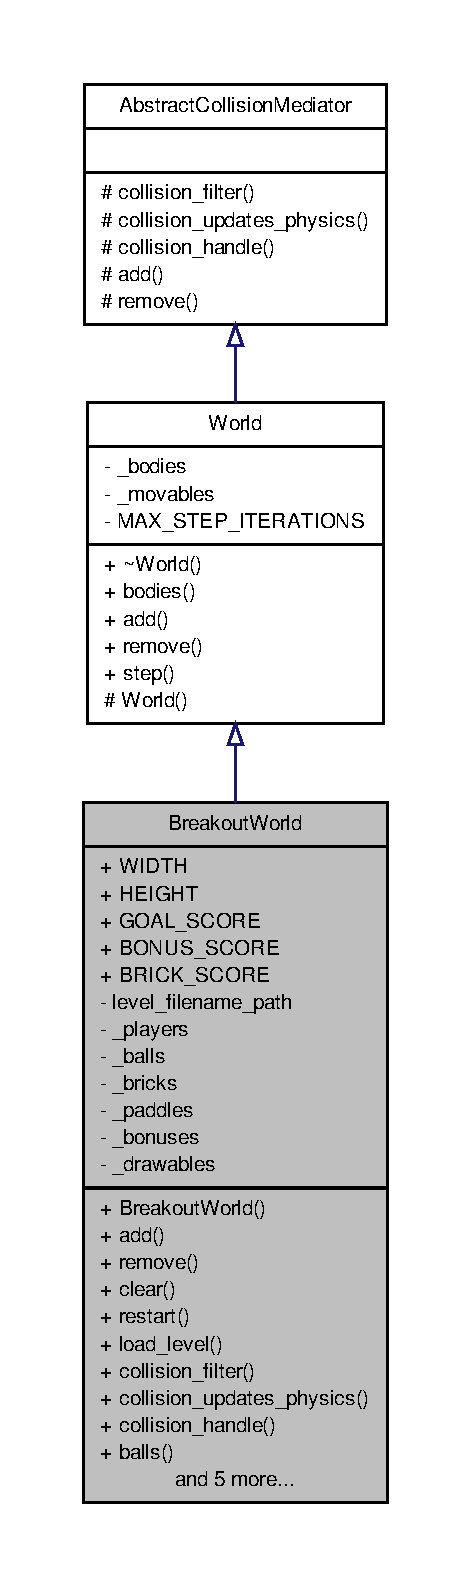
\includepdf[pages=-,scale=.8,pagecommand={}]{images/class_breakout_world__inherit__graph.pdf}
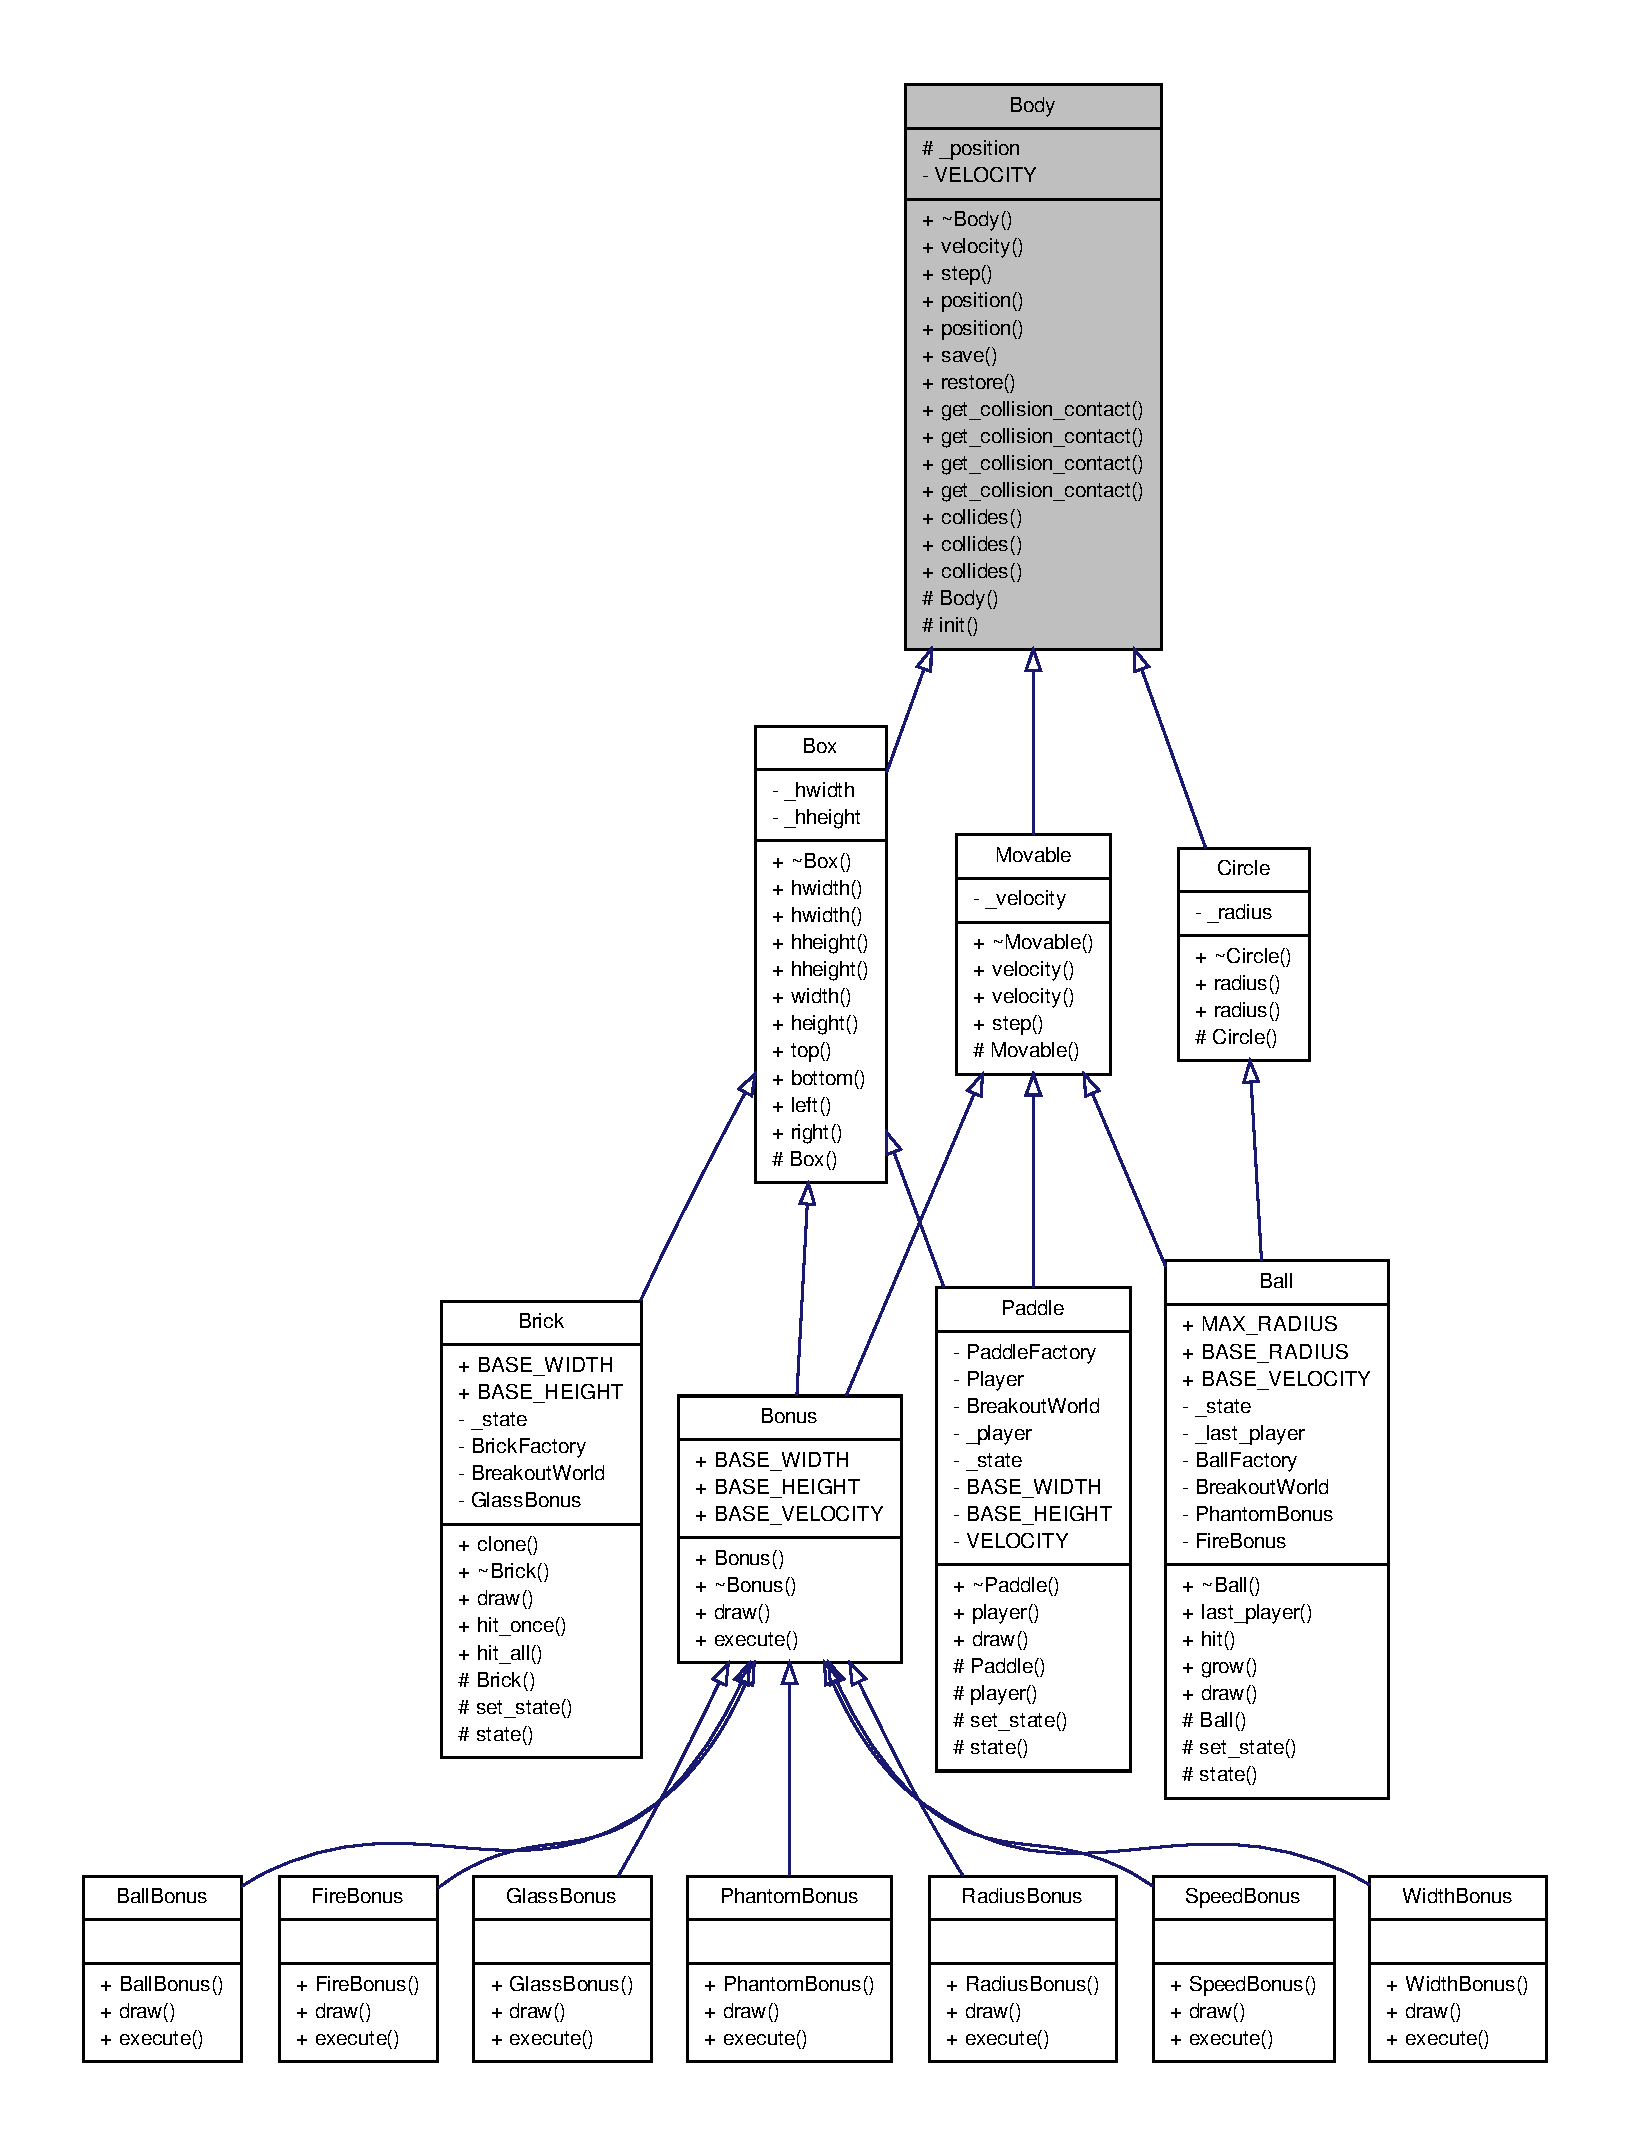
\includepdf[pages=-,scale=.8,pagecommand={}]{images/class_body__inherit__graph.pdf}
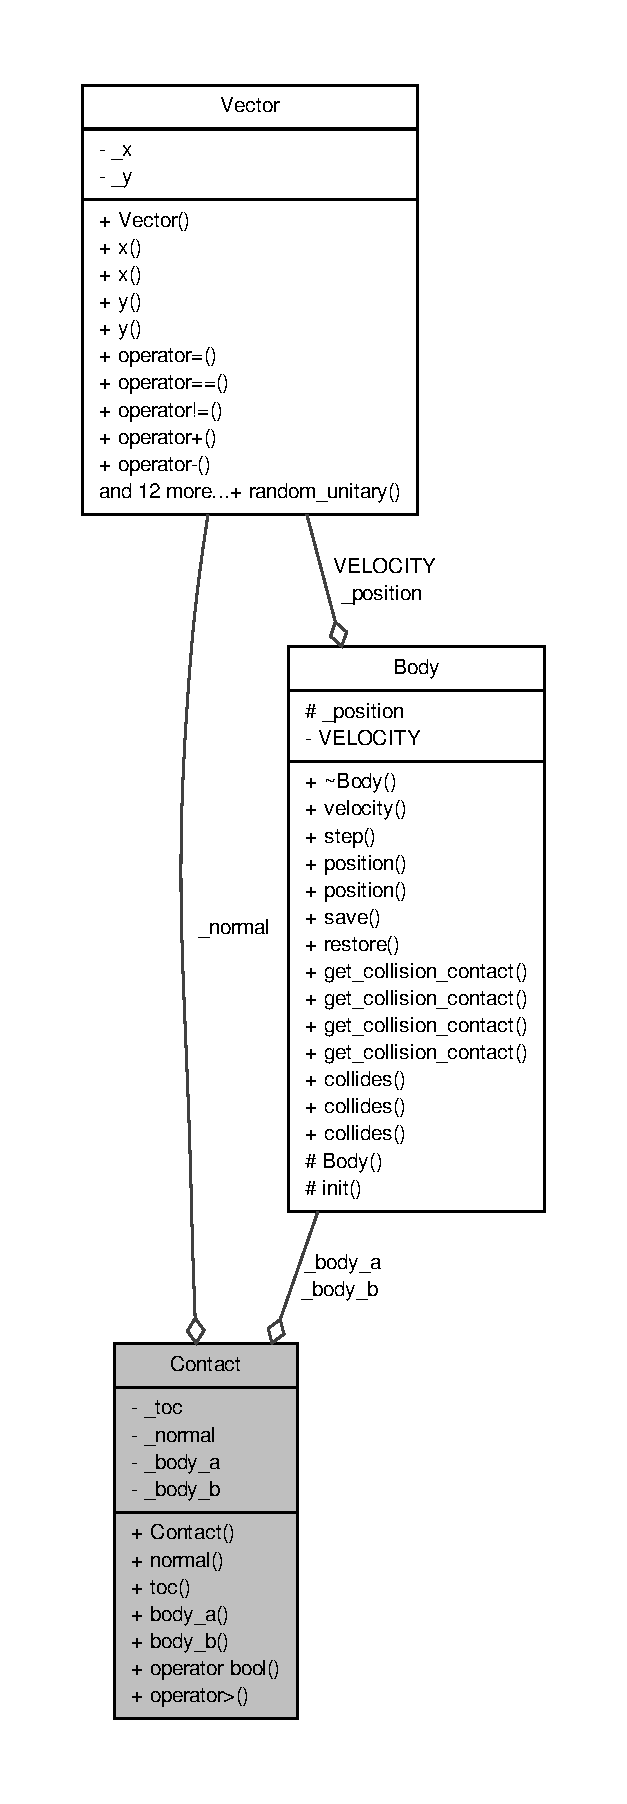
\includepdf[pages=-,scale=.8,pagecommand={}]{images/class_contact__coll__graph.pdf}
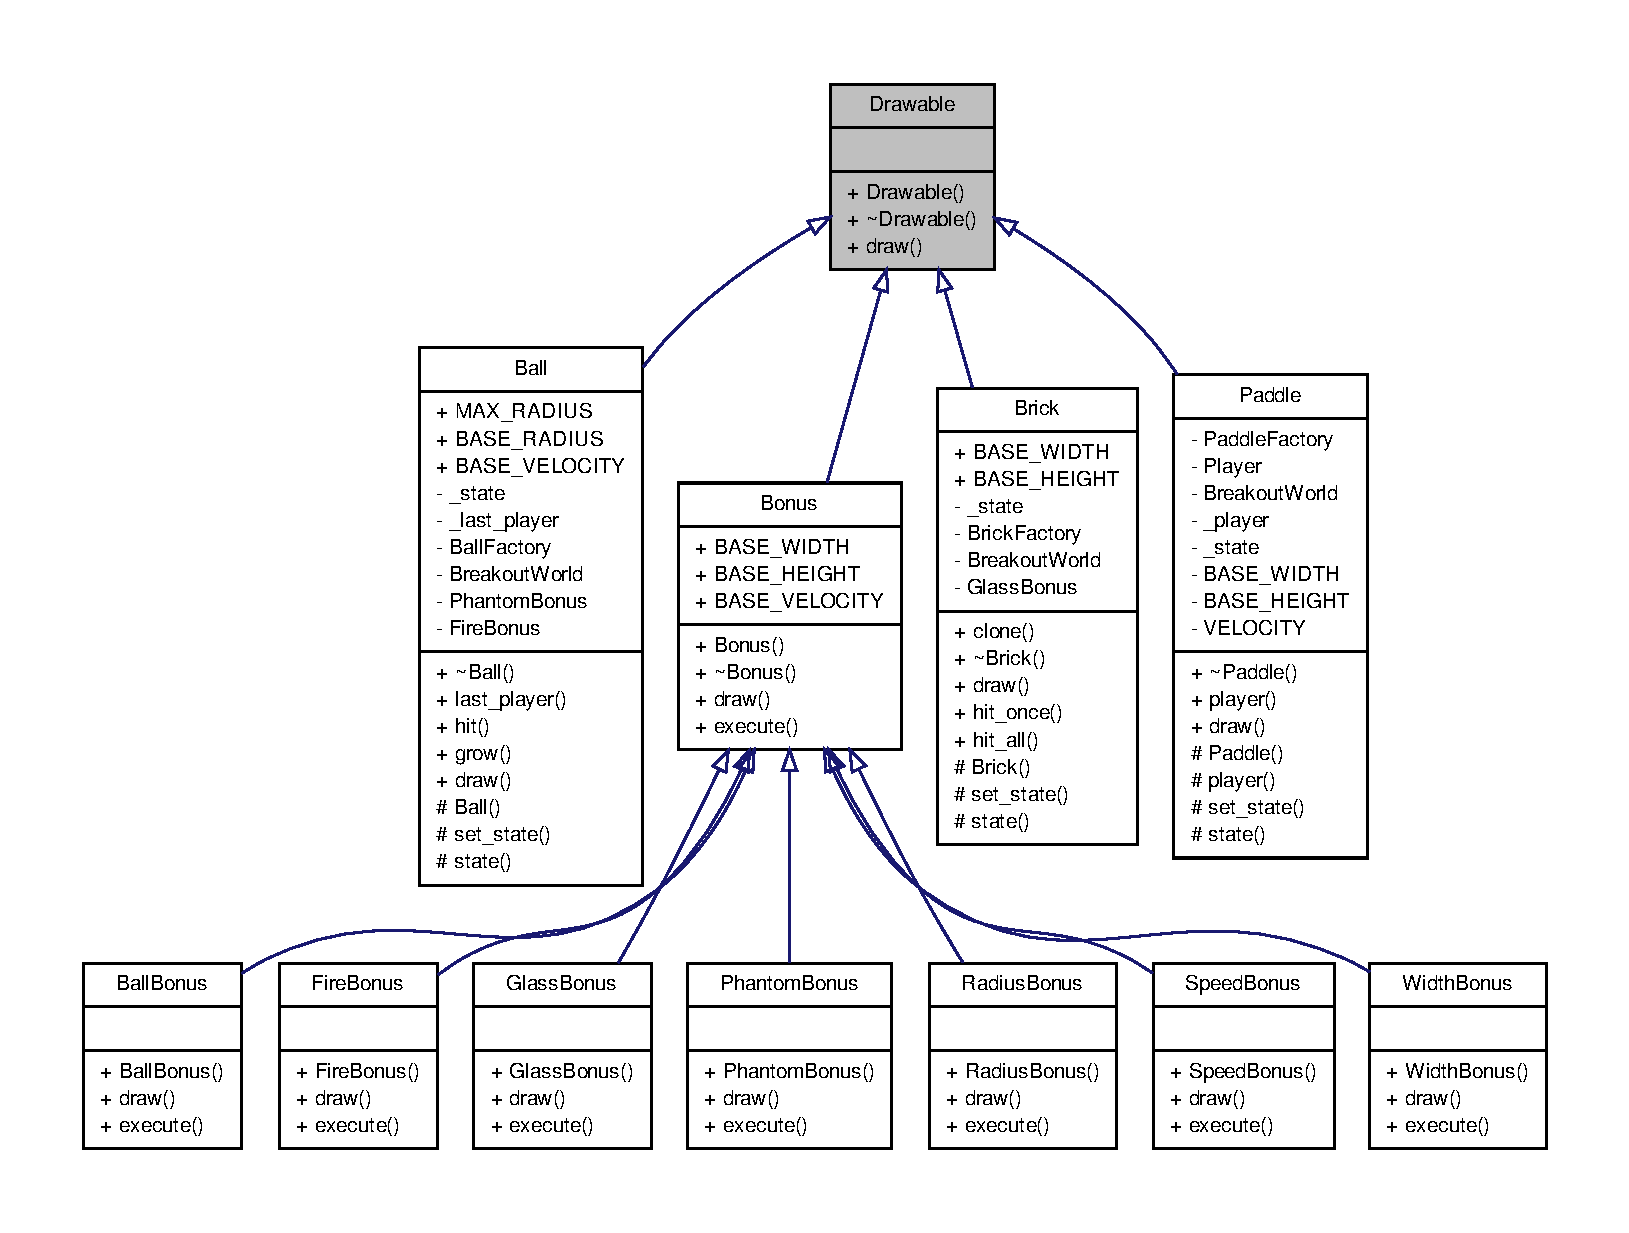
\includepdf[pages=-,scale=.8,pagecommand={}]{images/class_drawable__inherit__graph.pdf}
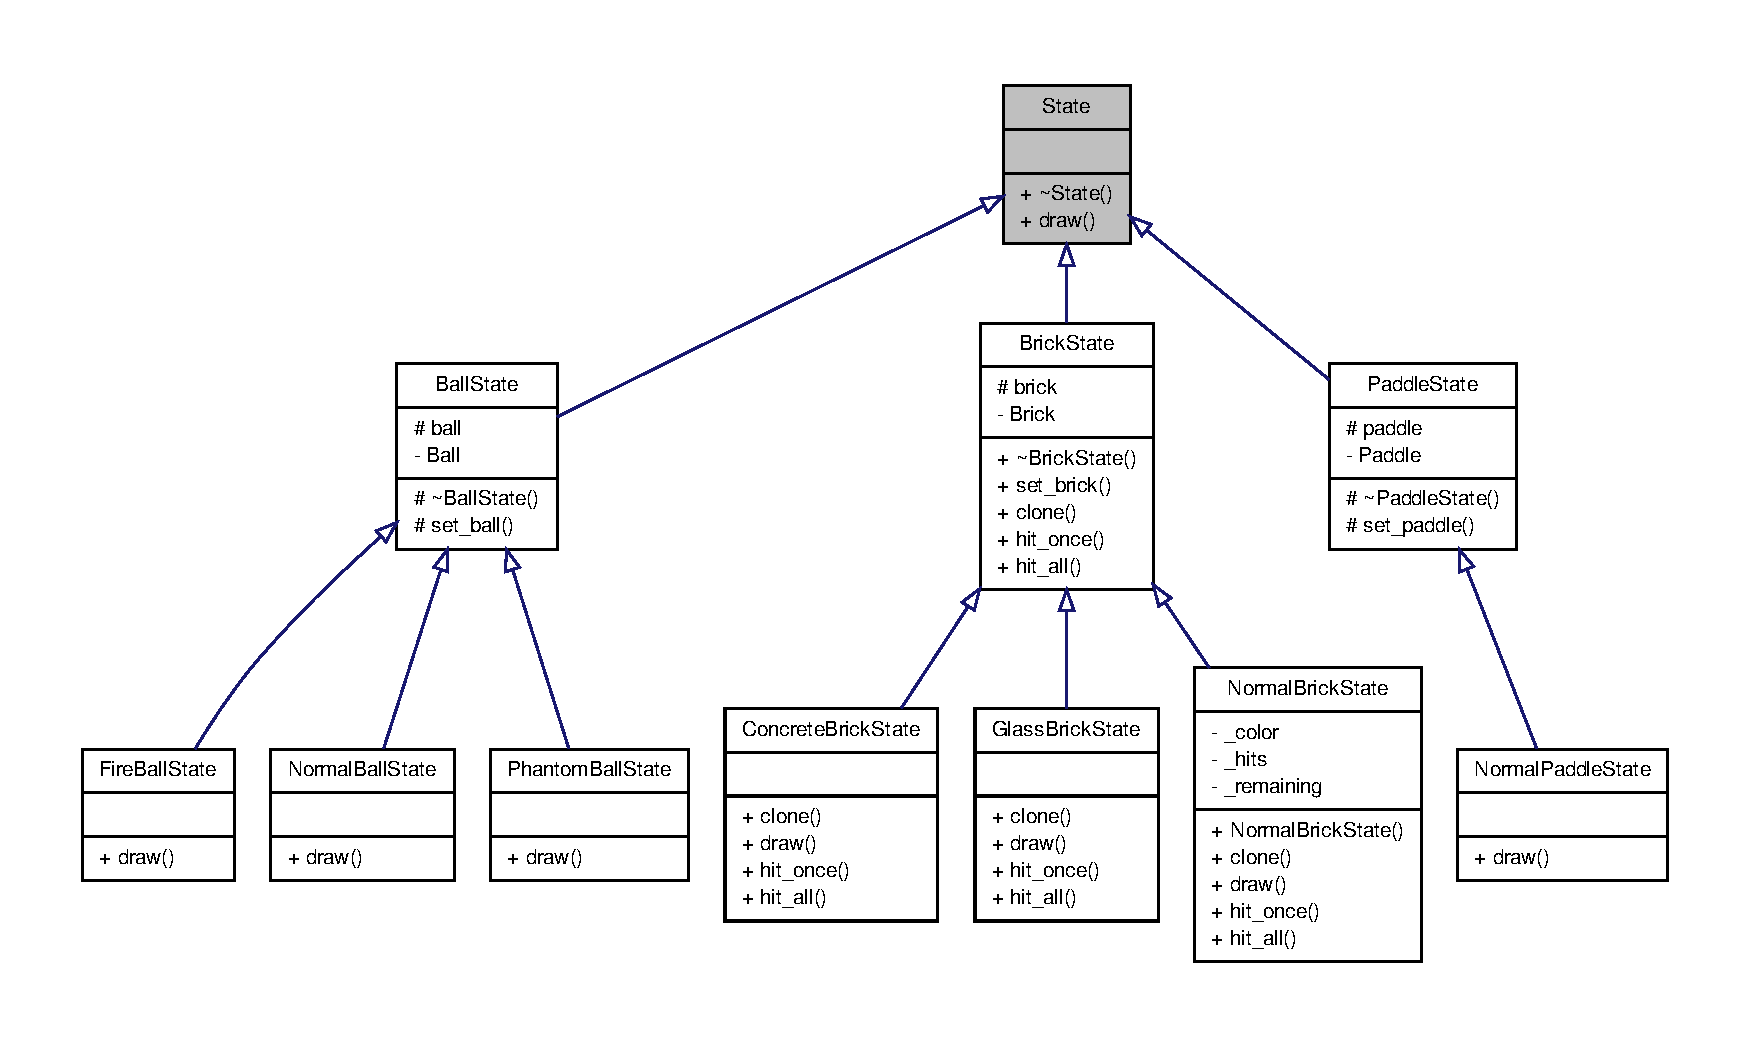
\includepdf[pages=-,scale=.8,pagecommand={}]{images/class_state__inherit__graph.pdf}
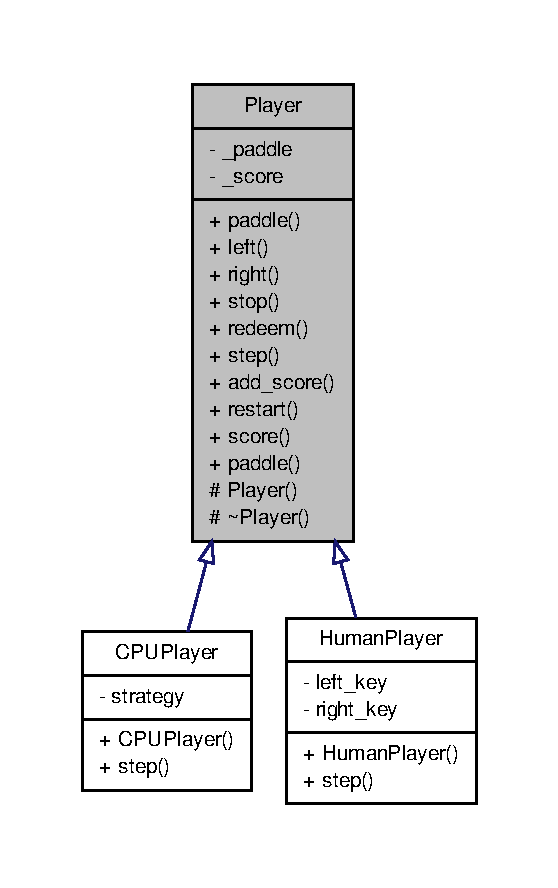
\includepdf[pages=-,scale=.8,pagecommand={}]{images/class_player__inherit__graph.pdf}
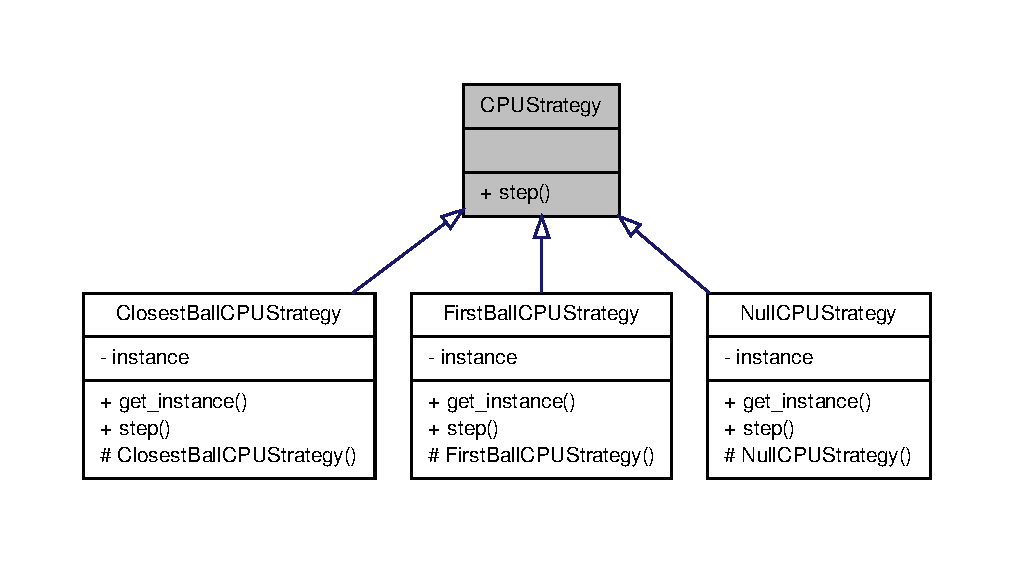
\includepdf[pages=-,scale=.8,pagecommand={}]{images/class_c_p_u_strategy__inherit__graph.pdf}
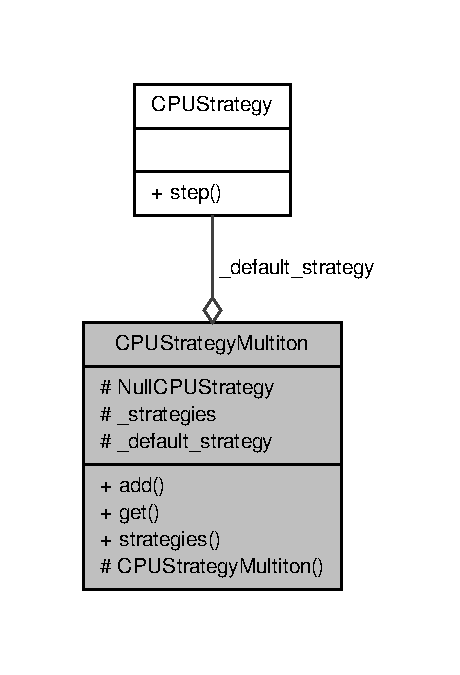
\includepdf[pages=-,scale=.8,pagecommand={}]{images/class_c_p_u_strategy_multiton__coll__graph.pdf}
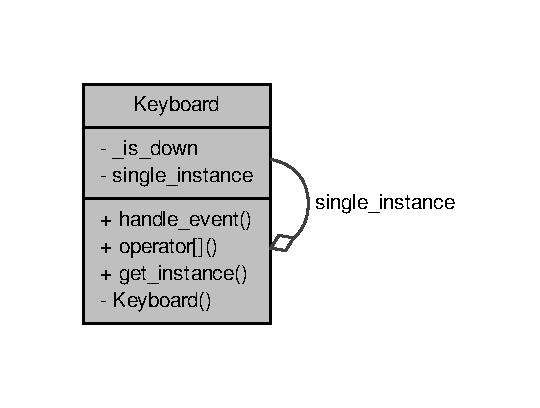
\includepdf[pages=-,scale=.8,pagecommand={}]{images/class_keyboard__coll__graph.pdf}

\end{document}
